\section{A Shift in System Design}
\label{sec:background:soa}

% Small introduction an how it relates to prev chapter.
% Docker ->  Small deployment cost -> next level soa
In the previous section, we introduced \glspl{container} technology and \Gls{docker} (\cref{sec:background:containers}). These technologies reduced the cost of deployment by introducing a small, standardized unit of software. The adoption of container technology led to a shift in architectural design and led to an increase in usage of \glsfirst{soa} design patterns. Due to the little overhead in terms of system resources caused by the \gls{container} technology, it was an ideal candidate for independent self-contained components. This section will introduce the concept of a logical \textit{service} in distributed systems and documents the general trends caused by the shift in architectural paradigms.

% Before SOA, monoliths
\subsection{The Software Monolith}
\label{sec:background:soa:monolith}

\begin{figure}[!t]
    \centering
    
    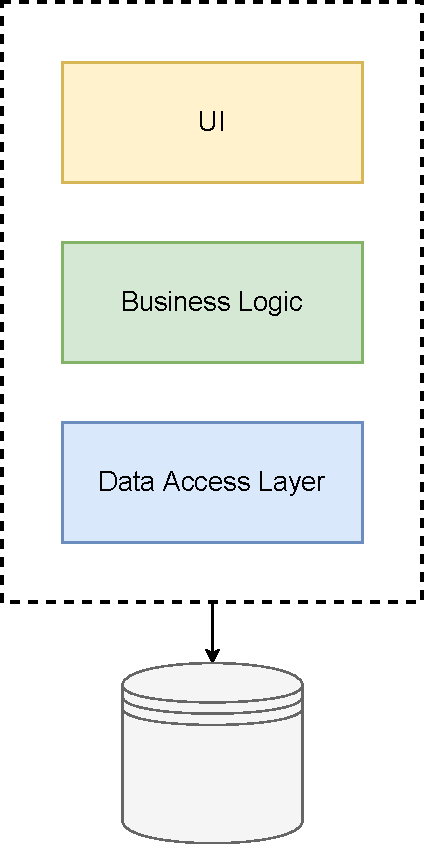
\includegraphics[width=0.3\linewidth]{2_background/figures/monolith-architecture.pdf}

    \caption[A monolithic software architecture.]{A monolithic architecture. In this form of software design, all the software is contained into a single, self-contained software program depicted by the dashed line. }
    \label{fig:monolithic-architecture}
\end{figure}


Before the adoption of \gls{soa} principles and the notion of services in general, companies, and organizations alike used to create so-called software \glspl{monolith}. A monolithic approach in software design produces a self-contained software program where all of its dependencies, data access patterns and user interfacing components are combined (as depicted in \cref{fig:monolithic-architecture}). This makes monolithic architectures difficult to use in distributed systems without ad-hoc solutions or frameworks \cite{dragoni2017microservices}. A software \gls{monolith} can have several advantages, it produces a single binary, all code is colocated together,  and it is a battle-tested architecture. However, it can also have several disadvantages, it can be hard to maintain, codebases can become gigantic over time and lead to accumulated technical debt that makes the product unmaintainable with reasonable efforts \cite{fritzsch2018monolith}. This architectural pattern also forces the developers of the application to stick to their technical architecture, such as the choice of programming language and frameworks used. Furthermore, it can suffer from dependency hell, where updating or adding libraries can break existing systems  \cite{merkel2014docker}. Finally, the architecture does not scale very well, by scaling the application every single aspect or module has to be duplicated which is inefficient if only a subset of the application is put under load.



\subsection{A Service-Oriented Approach}
\label{sec:background:soa:service-oriented}


\begin{figure}[!t]
    \centering
    
    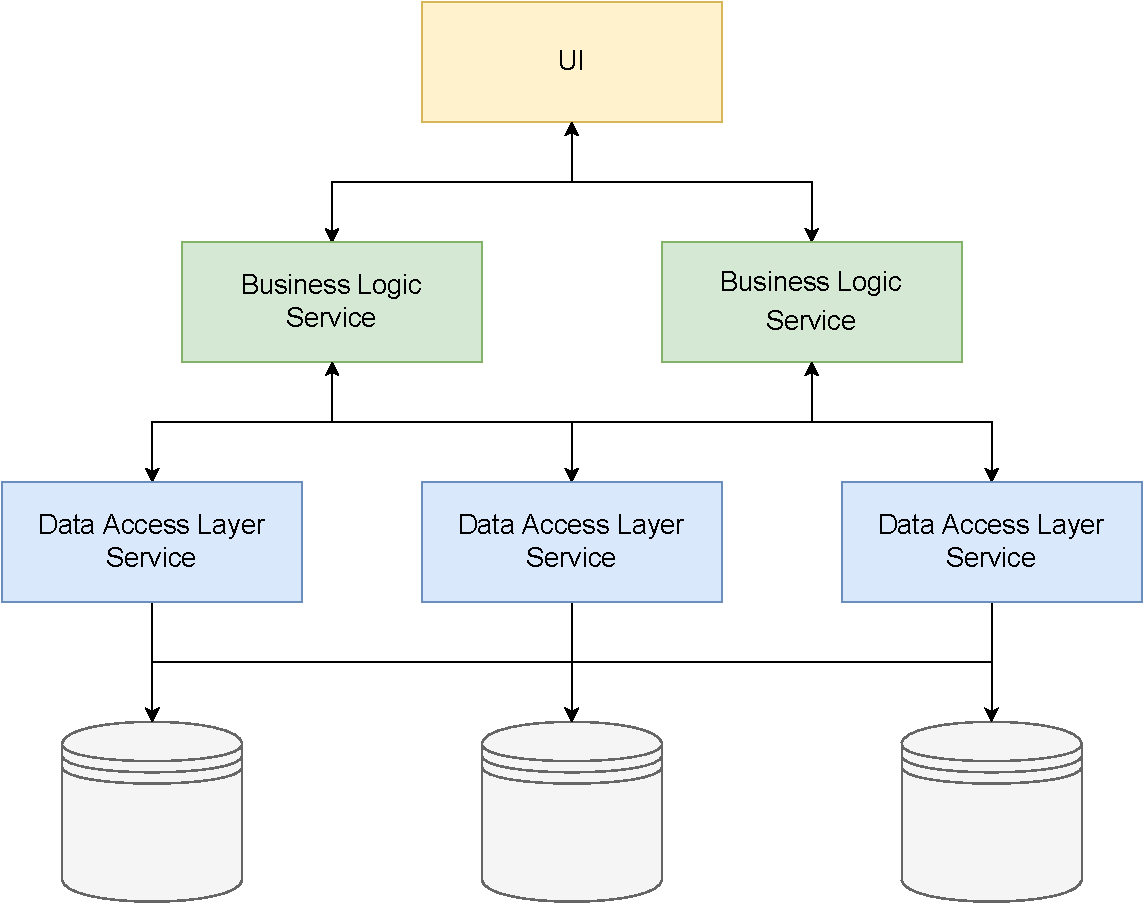
\includegraphics[width=.8\linewidth]{2_background/figures/service-oriented-architecture.pdf}

    \caption[A service-oriented software architecture.]{A service-oriented approach. This architectural approach allows engineers to split applications into separate business components which enables them to scale and operate individually.}
    \label{fig:soa-architecture}
\end{figure}


% From monolith to SOA
% - Benefits
% - Microservices
As previously stated, the \gls{monolith}ic architecture was not well suited for use in distributed systems. This led to a newer style of software architectures that decomposed the business logic into  logical \textit{services}, where functionalities are encapsulated and abstracted from context \cite{perrey2003service}. This architectural paradigm meant that applications have to be decomposed into several self-contained units, which are then exposed via a \textit{service interface}. The service interface utilizes common communication standards so that it can be incorporated in new applications without much hassle \cite{ibm-soa}. Each service contains the code and data integrations required to execute a discrete business function. The core idea behind the \gls{soa} paradigm is that it promotes reusability and component sharing. This then translates into several benefits, such as an increase in scalability because it allows for scaling at a service level instead of having to scale an entire monolith. Furthermore, it allows software developers to use multiple technologies and frameworks, making it easier to pick the right tools for the job. This is enabled by the fact that services can exchange data over common protocols and agreed upon data representations, such as \gls{json} for example.


\subsection{Microservices}
\label{sec:background:soa:microservices}

% Intrdouce Microservices
% Small recap of why now

\begin{figure}[!t]
    \centering
    
    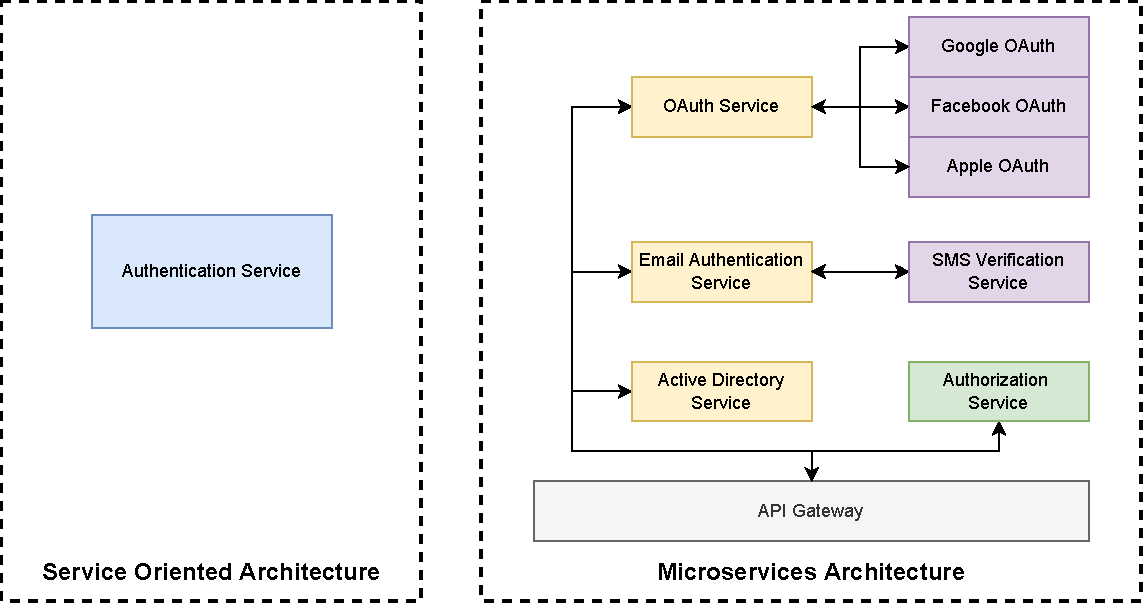
\includegraphics[width=.8\linewidth]{2_background/figures/microservices-vs-soa.pdf}

    \caption[The granularity of a microservices architecture.]{Service-Oriented architecture vs. microservices architecture both depicting an authentication service. Note: The granularity of the service definition depicts the most significant difference in the evolution of design.}
    \label{fig:soa-vs-microservices}
\end{figure}

The \textit{microservices} architecture (\cref{fig:soa-vs-microservices}) is an architectural style that emerged from the \gls{soa}. This evolvement was pushed by the  \gls{devops} movement and enabled by the decrease in deployment costs from the emerging \gls{container} technology \cite{amaral2015performance}.  The term \textit{microservice} dates in the context of distributed systems dates at least as far back as 2013 \cite{fowler-microservices}. It realizes its distinct itself from the \gls{soa}  paradigm by having a strong focus on its degree of independence regarding development and operation \cite{ibm-soa-vs-microservices}. The services that make up a \gls{soa}, can range from small, specialized services to enterprise-wide services, whereas a microservice consists of a highly specialized service, designed to do one thing well. This finer granularity allows for individual teams focussing on select subsets of an application and increases agility and development speed. However, this amplifies the problems that were mentioned above as it introduces more individual units in a complex system. Large companies such as Netflix that use such a microservices' architecture for example have reportedly managed to accumulate over 1000 microservices as of 2021 \cite{design-example-microservices, netflix-microservices-cost}.



\subsection{A New Set of Challenges}
\label{sec:background:soa:challenges}

% Down sides of a service oriented approach
% - Complexity
% - Network failures
% - Load balancing
% - Health cheecking
% - Serbice discovery
% Solutions to these complexitis
% - Fat clients
% - Enterprise Service Bus


\begin{figure}[!t]
    \centering
    
    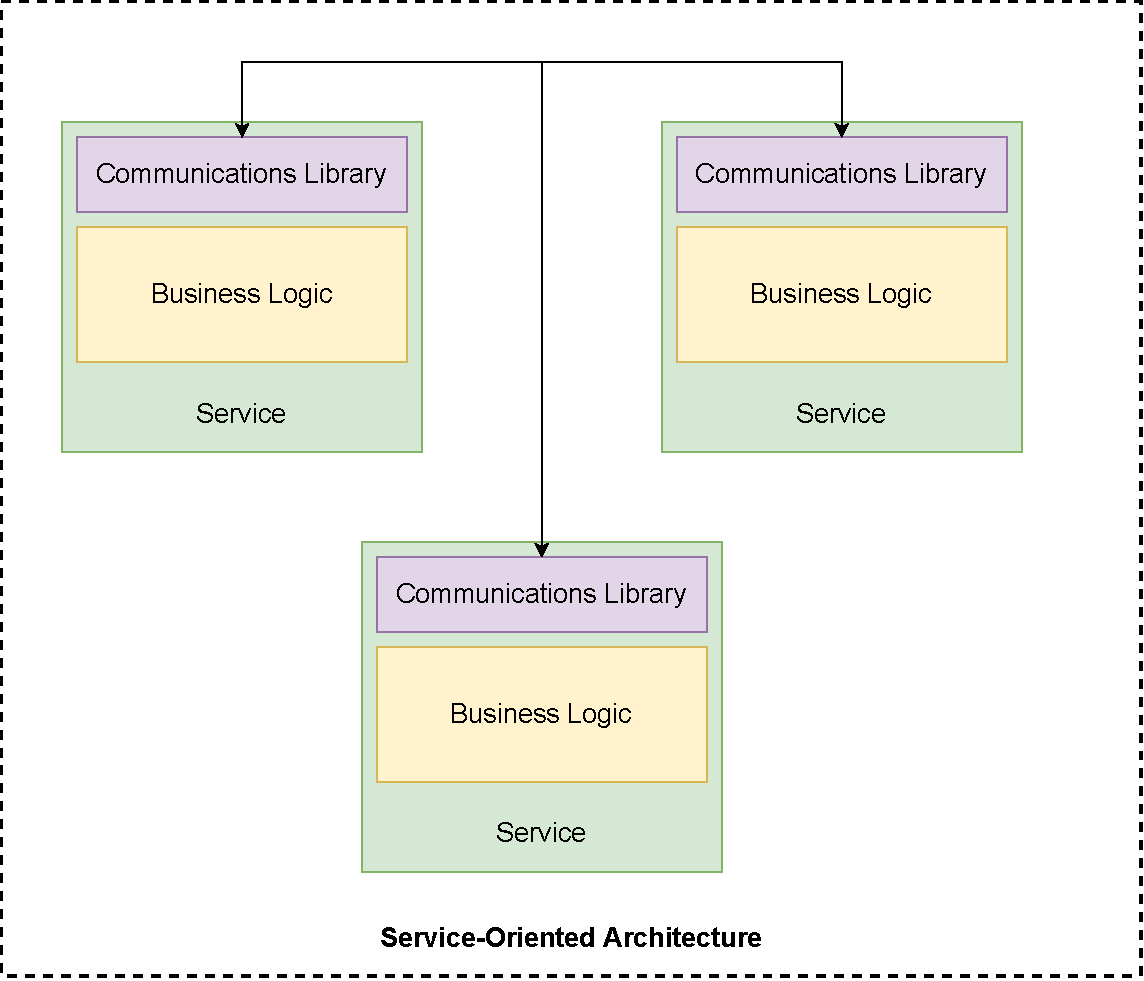
\includegraphics[width=.7\linewidth]{2_background/figures/software-lib-approach.pdf}

    \caption[Software library approach for solving networking challenges.]{Software library approach for solving the challenges introduces by a service-oriented design. In this design, the software library implements a uniform client and server API, designed to  handle fault tolerance, load balancing and latency optimizations to construct high-concurrency services.}
    \label{fig:software-lib-approach}
\end{figure}

However, by splitting the application up into several components, we introduce additional complexities. First off, the coarse granularity of the service-oriented design means that testing and validating every combination and condition may be very complex or even impossible \cite{mahmood2007service}. Furthermore, the loosely coupled services might be an architect's dream; however, it introduces additional complexities for a software developer \cite{fowler2012patterns}. Additionally, the service-to-service communications can now introduce failures, especially if they are carried out over unreliable networks such as the internet. Finally, the interoperability of services introduces additional challenges. How and where can we reach the services? Which version of the service is running and is it still compatible with everything? If there are multiple instances of this service, which one should be targetted to prevent overloading and ensure equal load? 



One approach used to solve these problems was through software libraries to handle all service-to-service communications (\cref{fig:software-lib-approach}) in a uniform way \cite{service-mesh-history}. Companies like Google, Netflix, and Twitter developed custom software libraries for this, such as \textit{Stubby} \cite{stubby}, \textit{Hystrix} \cite{hystrix} and \textit{Finagle} \cite{finagle} respectively. These libraries would perform load balancing, implement retry mechanisms, routing, and telemetry. A downside of this approach was that this meant that the libraries were usually written in a single programming language, locking the developers in, or resulting in having to support multiple libraries. Furthermore, it resulted in a scenario where updating the library meant that every service implementing it also required an update. 

% \todo{double check ESB bit} Another approach used was to utilize another design pattern that implements an \gls{esb}, an open standards, message-based, distributed integration infrastructure that provides routing, invocation and mediation services to facilitate the interactions of disparate distributed applications and services in a secure and reliable manner \cite{menge2007enterprise}. This dedicated piece of infrastructure combines  Message-Oriented Middleware (MOM), web services, transformation and routing intelligence as a backbone for Service-Oriented Architecture.


